\chapter{Annex}\label{sec:irgendwas}

\section{Latent Space Dimension}

In the process of selecting the autoencoder architecture, a comparison was made between sizes in the latent space. The goal was to encode the segment descriptions with as small a dimensionality as possible, in order to show that the autoencoder could perform better than other descriptors even for similar description sizes. Another advantage of keeping descriptions small is that they would require less storage space when running SegMatch on long datasets.\\

Non-trivial improvements in reconstruction quality were observed when switching from a latent space size of 10 to 15. However, larger dimensionalities showed increased redundancies in the latent space (such as unused dimensions, discussed in Chapter \ref{chap:ae}, Section \ref{sec:ae-results}, or lack of insignificant improvements in reconstruction ability).\\

As an extremum example, a model with a 2-dimensional latent space was trained similarly to the regular models. The distribution of segment descriptions in this 2D space is shown in Fig.~\ref{fig:2d_latent_space}. The model's reconstruction abilities were observed as quite limited, often failing to produce a reconstruction, or reconstructing segments of a certain class as 3D clusters resembling segments of an entirely different class. In accordance with this, there is much overlap between classes visible in Fig.~\ref{fig:2d_latent_space}.\\

\begin{figure}
  \centering
  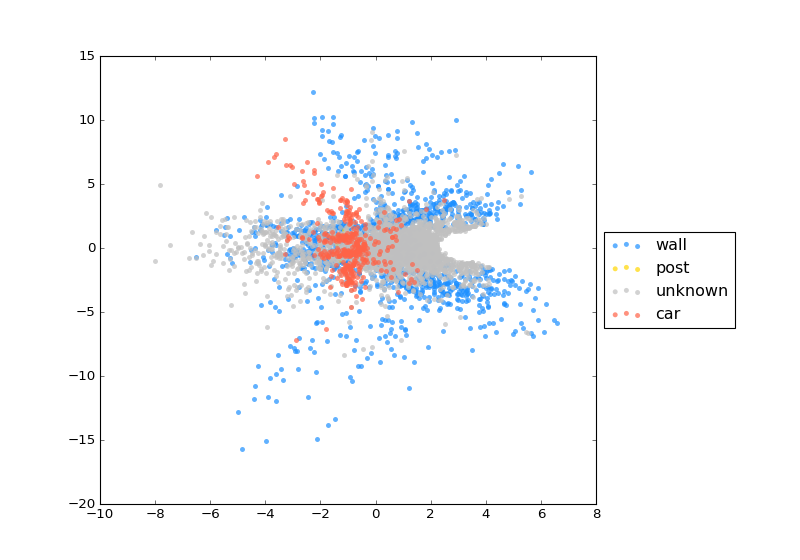
\includegraphics[width=5.2in]{images/2dlatentspace.png}
  \caption{Segment descriptions given by a 2-dimension latent space autoencoder model}
  \label{fig:2d_latent_space}
\end{figure}
